\documentclass{cmn}

\def\imm{12}
\def\rs{5}
\def\funct{3}
\def\rd{5}
\def\opcode{7}
\def\mag{3}

\begin{document}
  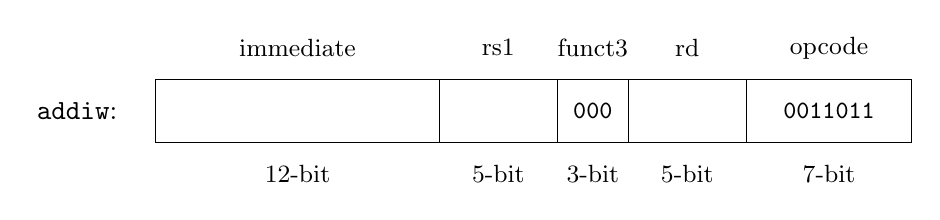
\begin{tikzpicture}
    \node at (-10mm,4mm) {\texttt{addiw}:};

    \draw (0,0) -- ++(96mm,0) -- ++(0,8mm) -- ++(-96mm,0) -- cycle;
    \draw ({\imm*\mag*1mm},0) -- ++(0,8mm);
    \draw ({(\imm+\rs)*\mag*1mm},0) -- ++(0,8mm);
    \draw ({(\imm+\rs+\funct)*\mag*1mm},0) -- ++(0,8mm);
    \draw ({(\imm+\rs+\funct+\rd)*\mag*1mm},0) -- ++(0,8mm);

    \node at ({0.5*\imm*\mag*1mm},12mm) {\small immediate};
    \node at ({(\imm+0.5*\rs)*\mag*1mm},12mm) {\small rs1};
    \node at ({(\imm+\rs+0.5*\funct)*\mag*1mm},12mm) {\small funct3};
    \node at ({(\imm+\rs+\funct+0.5*\rd)*\mag*1mm},12mm) {\small rd};
    \node at ({(\imm+\rs+\funct+\rd+0.5*\opcode)*\mag*1mm},12mm) {\small opcode};

    \node at ({(\imm+\rs+0.5*\funct)*\mag*1mm},4mm) {\small\texttt{000}};
    \node at ({(\imm+\rs+\funct+\rd+0.5*\opcode)*\mag*1mm},4mm) {\small\texttt{0011011}};

    \node at ({0.5*\imm*\mag*1mm},-4mm) {\small 12-bit};
    \node at ({(\imm+0.5*\rs)*\mag*1mm},-4mm) {\small 5-bit};
    \node at ({(\imm+\rs+0.5*\funct)*\mag*1mm},-4mm) {\small 3-bit};
    \node at ({(\imm+\rs+\funct+0.5*\rd)*\mag*1mm},-4mm) {\small 5-bit};
    \node at ({(\imm+\rs+\funct+\rd+0.5*\opcode)*\mag*1mm},-4mm) {\small 7-bit};
  \end{tikzpicture}
\end{document}
